% JUMP TO LINE 60, 73
\documentclass[preview, margin=0.6in]{standalone}
\usepackage[letterpaper,portrait,top=0.4in, left=0.6in, right=0.6in, bottom=1in]{geometry}

\usepackage{amsmath, amsfonts, amsthm, amssymb}
\usepackage{graphicx, float}
\usepackage{mathtools}
\usepackage{titlesec}
\usepackage{interval}
\usepackage{hyperref}
\usepackage{siunitx}
\usepackage{titling}
\usepackage{vwcol}
\usepackage{setspace}
\usepackage{empheq}
\usepackage{cancel}
\usepackage{esdiff}
\usepackage{multicol}
\usepackage{mdframed}
\usepackage{esdiff}
\usepackage{tikzsymbols}
\usepackage{multicol}
\usepackage{tikz}
\usepackage{varwidth}
\usepackage{pgfplots}
\pgfplotsset{compat=1.18}
\intervalconfig {
	soft open fences
}

\newcommand{\alignedintertext}[1]{%
  \noalign{%
    \vskip\belowdisplayshortskip
    \vtop{\hsize=\linewidth#1\par
    \expandafter}%
    \expandafter\prevdepth\the\prevdepth
  }%
}

\newtheorem{lemma}{Lemma}

\renewcommand{\qedsymbol}{\Smiley[1.3]}
\newcommand*{\problem}[1]{\section*{Problem #1}}
\newcommand*{\aps}{\section*{AP Corner}}
\newcommand*{\deriv}[1][x]{\ensuremath{\dfrac{\mathrm{d}}{\mathrm{d}#1}}}
\newcommand*{\floor}[1]{\ensuremath{\lfloor #1\rfloor}}
\newcommand*{\lheqzero}{\ensuremath{\underset{\text{L'H}}{\overset{\left[\frac00\right]}{=}}}}
\newcommand*{\lheqinfty}{\ensuremath{\underset{\text{L'H}}{\overset{\left[\frac{\infty}{\infty}\right]}{=}}}}

\DeclareMathOperator{\DNE}{DNE}
\DeclareMathOperator{\sgn}{sgn}

\DeclareMathOperator{\arccsc}{arccsc}
\DeclareMathOperator{\arcsec}{arcsec}
\DeclareMathOperator{\arccot}{arccot}

\setlength{\parindent}{0pt}

%opening
\title{\vspace*{-30pt}Problem Set \#21}
\author{Jayden Li}
\date{\today}

% \allowdisplaybreaks
\postdisplaypenalty=100000

\begin{document}
\setstretch{1.25}
\fontsize{12pt}{12pt}\selectfont
\setlength{\abovedisplayskip}{0pt}
\maketitle
\problem{5}
\begin{itemize}
	\item[(a)]
		$\begin{aligned}[t]
			\text{area of 1 quadrant}
			&=\int_{0}^{a}\sqrt{b^2-\frac{b^2x^2}{a^2}}\,\mathrm{d}x
			=\int_{0}^{a}b\sqrt{1-\frac{x^2}{a^2}}\,\mathrm{d}x \\
			&=\left[\begin{aligned}
					x&=a\sin\theta \\
					\mathrm{d}x&=a\cos\theta \,\mathrm{d}\theta
			\end{aligned}\right]
			\int_{0}^{\pi/2}b \sqrt{1-\frac{a^2\sin^2\theta}{a^2}}\cdot a\cos\theta\,\mathrm{d}\theta
			=ab \int_{0}^{\pi/2}\cos^2\theta\,\mathrm{d}\theta \\
			&=ab \int_{0}^{\pi/2}\frac{1+\cos2\theta}{2}\,\mathrm{d}\theta
			=ab \cdot \frac12 \left[\theta+\frac{\sin2\theta}{2}\right]_{0}^{\pi/2}
			=\frac{ab}{2}\left(\frac{\pi}{2}+0-0-0\right)
			=\frac{\pi ab}{4} \\
			\text{area}
			&=4\cdot\text{area of 1 quadrant}
			=4\cdot \frac{\pi ab}{4}
			=\boxed{\pi ab}
		\end{aligned}$

	\item[(b)]
		Circle is larger than ellipse.

		Area of an ellipse with semi-axes $a$ and $a-b$ is $\pi a(a-b)$.

		$\begin{aligned}[t]
			A_{\text{between circle and ellipse}}
			&=A_{\text{circle}}-A_{\text{ellipse}}
			=\pi a^2-\pi ab
			=\pi a(a-b)
			=S_{\text{other ellipse}}
		\end{aligned}$
\end{itemize}

\problem{6}
\begin{center}
	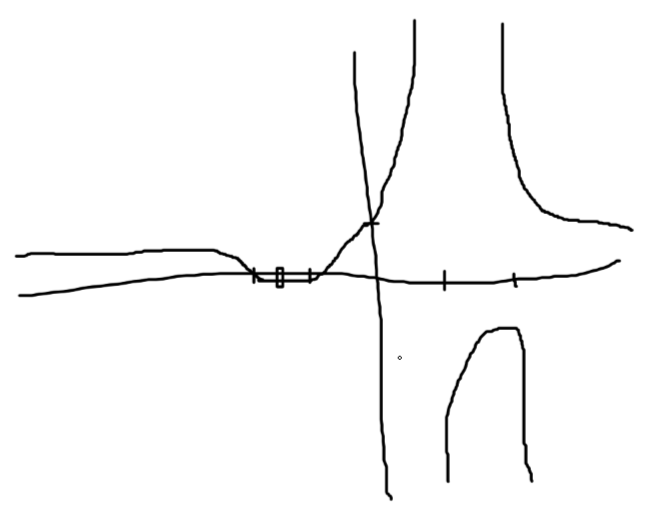
\includegraphics[width=0.5\linewidth]{q6.png}
\end{center}
$\begin{aligned}[t]
	\text{signed area}
	&=\int_{-2}^{-1}\frac{x^2+3x+2}{x^2-3x+2}\,\mathrm{d}x
	=\int_{-2}^{-1}\left(1+\frac{6x}{(x-1)(x-2)}\right)\mathrm{d}x
	=\int_{-2}^{-1}\left(1+\frac{A}{x-1}+\frac{B}{x-2}\right)\mathrm{d}x \\
	\alignedintertext{
		\begin{mdframed}
			$\begin{aligned}[t]
				\frac{A}{x-1}+\frac{B}{x-2}
				&=\frac{6x}{x^2-3x+2}
				\implies \frac{Ax-2A+Bx-B}{x^2-3x+2}=\frac{6x}{x^2-3x+2}
				=\left\{\begin{aligned}
						A+B&=6 \\
						-2A-B&=0
				\end{aligned}\right. \\
				&\implies -A=6
				\implies A=-6
				\implies B=12
			\end{aligned}$
		\end{mdframed}
	}
	&=\int_{-2}^{-1}\left(1-\frac{6}{x-1}+\frac{12}{x-2}\right)\mathrm{d}x
	=\Big[x-6\ln|x-1|+12\ln|x-2|\Big]_{-2}^{-1} \\
	&=-1-6\ln2+12\ln3-\left(-2-6\ln3+12\ln4\right)
	=-1-6\ln2+12\ln3+2+6\ln3-12\ln4 \\
	&=1-6\ln2+18\ln3-24\ln2
	=1-30\ln2+18\ln3
	=1-6 \left(5\ln2-3\ln 3\right) \\
	&=1-6 \left(\ln \left(2^5\right)-\ln \left(3^3\right)\right)
	=1-6\ln \left(\frac{2^5}{3^3}\right)
	=1-6\ln \left(\frac{32}{27}\right) \\
	\text{area}
	&=\left|\text{signed area}\right|
	=\left|1-6 \ln\left(\frac{32}{27}\right)\right|
	=\boxed{6 \ln\left(\frac{32}{27}\right)-1}
\end{aligned}$

\problem{7}
\begin{center}
	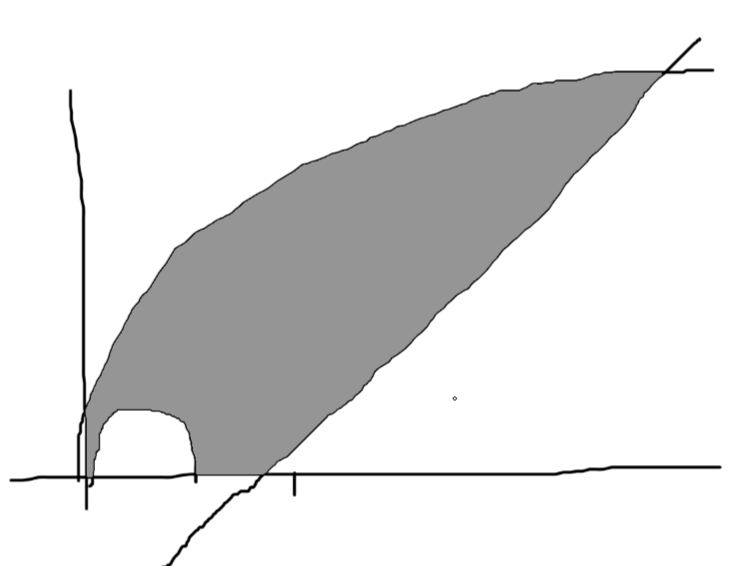
\includegraphics[width=0.5\linewidth]{q7.png}
\end{center}
We integrate with respect to $y$ because it is easier. We need to find the upper bound of integration.

$\begin{aligned}[t]
    \frac{y^2}{4}=y+2
	&\implies y^2=4y+8
	\implies y^2-4y-8=0
	\implies y=\frac{4\pm \sqrt{16+32}}{2}
	\implies y=\frac{4\pm 2 \sqrt{12}}{2} \\
	&\implies y=2\pm \sqrt{12}
\end{aligned}$

We only care care about first quadrant, so we keep $y=2+\sqrt{12}$.

Equation of the circle is $x^2+y^2=2x\implies (x-1)^2+y^2=1$. Radius of circle is $1$.

$\begin{aligned}[t]
	S_{\text{semicircle}}&=\frac12\cdot\pi(1)^2=\frac{\pi}{2} \\
	S_{\text{other}}&=\int_{0}^{2+\sqrt{12}}\left(y+2-\frac{y^2}{4}\right)\mathrm{d}y
	=\int_{0}^{2+2 \sqrt{3}}\left(y+2-\frac{y^2}{4}\right)\mathrm{d}y
	=\left[\frac{y^2}{2}+2y-\frac{y^3}{12}\right]_{0}^{2+2 \sqrt{3}} \\
	&=\frac{\left(2+2 \sqrt{3}\right)^2}{2}+2\left(2+2 \sqrt{3}\right)-\frac{\left(2+2 \sqrt{3}\right)^3}{12}
	=2\left(1+\sqrt{3}\right)^2+4\left(1+\sqrt{3}\right)-\frac{2\left(1+\sqrt{3}\right)^3}{3} \\
	S&=S_{\text{other}}-S_{\text{semicircle}}=\boxed{2\left(1+\sqrt{3}\right)^2+4\left(1+\sqrt{3}\right)-\frac{2\left(1+\sqrt{3}\right)^3}{3}-\frac{\pi}{2}}
\end{aligned}$

\textit{(this is equivalent to the answer given on the set, but I can't figure out how to simplify)}

\problem{8}
In the picture below, the green line is $x=0$, red is $y=f(x)=\sqrt{\tan x}$, purple is $x=a$, and blue is $y=f(c)=\sqrt{\tan c}$.

\begin{center}
	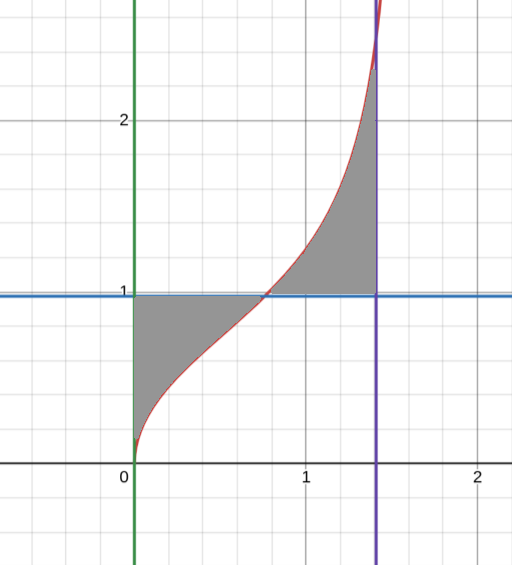
\includegraphics[width=0.5\linewidth]{q8.png}
\end{center}

$\begin{aligned}[t]
	A
	&=\int_{0}^{c}\left(f(c)-f(x)\right)\mathrm{d}x+\int_{c}^{a}\left(f(x)-f(c)\right)\,\mathrm{d}x
	=\int_{0}^{c}f(c)\,\mathrm{d}x-\int_{0}^{c}f(x)\,\mathrm{d}x+\int_{c}^{a}f(x)\,\mathrm{d}x-\int_{c}^{a}f(c)\,\mathrm{d}x \\
	&=cf(c)-\int_{0}^{c}f(x)\,\mathrm{d}x+\int_{c}^{a}f(x)\,\mathrm{d}x-(a-c)f(c) \\
	\diff Ac
	&=\deriv[c]\left[cf(c)-\int_{0}^{c}f(x)\,\mathrm{d}x+\int_{c}^{a}f(x)\,\mathrm{d}x-(a-c)f(c)\right] \\
	0&=f(c)+cf'(c)-f(c)-f(c)-\left(-f(c)+(a-c)f'(c)\right)
	=cf'(c)-f(c)+f(c)-(a-c)f'(c) \\
	&=f'(c) \left(c-(a-c)\right)
	=\deriv[c]\left[\sqrt{\tan c}\right](c-a+c)
	=\frac{\sec^2c}{2 \sqrt{\tan c}}(2c-a) \\
	0&=\underbrace{\frac{1}{2 \cos^2(c) \sqrt{\tan c}}}_{\text{cannot equal $0$}}\underbrace{(2c-a)}_{\text{might equal $0$}}
	\implies 2c-a=0
	\implies c=\frac{a}{2}
\end{aligned}$
We also know that $\left.\diff[2]Ac\right|_{c=a/2}>0$ (by computer), which means that \boxed{c=a/2} is a minimum.

\problem{9}
The line $y=g(x)=f^{-1}(x)$ is equivalent to $x=f(y)$. The upper bound of integration is $y=f^{-1}(37)=3$ because $f(3)=37$.

$\begin{aligned}[t]
	\text{area}
	&=\int_{0}^{f^{-1}(37)}\left(37-f(y)\right)\mathrm{d}y
	=\int_{0}^{3}\left(37-y^3-3y-1\right)\mathrm{d}y
	=\int_{0}^{3}\left(36-y^3-3y\right)\mathrm{d}y \\
	&=\left[36y-\frac{y^4}{4}-\frac{3y^2}{2}\right]_{0}^{3}
	=108-\frac{81}{4}-\frac{27}{2}-0+0+0
	=\frac{432-81-54}{4}
	=\boxed{\frac{297}{4}}
\end{aligned}$

\end{document}
